% !TEX encoding = UTF-8
%Koma article
\documentclass[fontsize=12pt,paper=letter,twoside]{scrartcl}
\usepackage{graphicx}
\usepackage{multirow}

%Standard Pre-amble
\usepackage[top=4cm,bottom=4cm,left=3cm,right=3cm,asymmetric]{geometry}
%\geometry{landscape}                % Activate for for rotated page geometry
%\usepackage[parfill]{parskip}    % Begin paragraphs with an empty line rather than an indent
\usepackage[table,xcdraw]{xcolor}
\usepackage{graphicx}

\usepackage{amsmath}
\usepackage{amssymb}
\usepackage{epstopdf}
\DeclareGraphicsRule{.tif}{png}{.png}{`convert #1 `dirname #1`/`basename #1 .tif`.png}
% Listings needs package courier
\usepackage{listings} % Needs 
\usepackage{courier}

\usepackage[framemethod=TikZ]{mdframed}
\usepackage{url}

\usepackage{sty/bsymb} %% Event-B symbols
\usepackage{sty/eventB} %% REQ and ENV
\usepackage{sty/calculation}

%Maths
\usepackage{amssymb,amsmath}
\def\Fl{\mathbb{F}}
\def\Rl{\mathbb{R}}
\def\Nl{\mathbb{N}}
\def\Bl{\mathbb{B}}
\def\St{\mathbb{S}}
\newcommand{\ovr}{\upharpoonright}
\newcommand{\var}[1]{\textit{#1}}
%Useful definitions
\newcommand{\mv}[1]{\textit{m\_#1}}
\newcommand{\cv}[1]{\textit{c\_#1}}
\newcommand{\degree}[1]{^{\circ}\mathrm{#1}}
%\newcommand{\comment}[1]{{\footnotesize \quad\texttt{--}\textrm{#1}}}
\newcommand{\im}[1]{i\texttt{-\!#1}}

\usepackage[headsepline]{scrpage2}
\pagestyle{scrheadings}
\ihead[]{\small EECS4312 Report1}
\ohead[]{\small \thepage}
\cfoot[]{}
\ofoot[]{}


%%%%PVS environment%%%%%%%%%%%%%%%%%%%
\lstnewenvironment{pvs}[1][]
    {\lstset{#1,captionpos=b,language=pvs,
    mathescape=true,
    basicstyle=\small\ttfamily,
    numbers=none,
    frame=single,
    % numberstyle=\tiny\color{gray},
    % backgroundcolor=\color{lightgray},
    firstnumber=auto
    }}
    {}
 %%%%%%%%%%%%%%%%%%%%%%%%%%%%%%%%
 
%%%%Verbatim environment%%%%%%%%%%%%%%%%%%%
\lstnewenvironment{code}[1][]
    {\lstset{#1,captionpos=b,
    mathescape=true,
    basicstyle=\small\ttfamily,
    numbers=none,
    frame=single,
    % numberstyle=\tiny\color{gray},
    % backgroundcolor=\color{lightgray},
    firstnumber=auto
    }}
    {}

% \newenvironment{boxed}[1]
%    {\begin{center}
%    #1\\[1ex]
%    \begin{tabular}{|p{0.9\textwidth}|}
%    \hline\\
%    }
%    { 
%    \\\\\hline
%    \end{tabular} 
%    \end{center}
%    }
 %%%%%%%%%%%%%%%%%%%%%%%%%%%%%%%%
 
 %Text in a box
\newenvironment{textbox}
    {\begin{center}
    \begin{tabular}{|p{0.9\textwidth}|}
    \hline\\
    }
    { 
    \\\\\hline
    \end{tabular} 
    \end{center}
    }

\usepackage{hyperref}

%Highlight \hl{}
\usepackage{soul}

\usepackage{enumitem}
\newlist{mylist}{itemize}{1}
\setlist[mylist]{label=\textbullet,leftmargin=1cm,nosep}

\usepackage{multirow}

% Reduce space between figure and caption
%\usepackage{caption}
%\captionsetup[table]{font=small,skip=0pt}     %% Adjust here
%or equivalently 
\usepackage[font=small,skip=4pt]{caption}

% Set the header
\ihead[]{\small EECS4312 eHealth Project}
\title{EECS4312 eHealth Project}

%Useful definitions
%\newcommand{\mv}[1]{\textit{m\_#1}}
%\newcommand{\cv}[1]{\textit{c\_#1}}
%\newcommand{\degree}[1]{^{\circ}\mathrm{#1}}
%\newcommand{\comment}[1]{{\footnotesize \quad\texttt{--}\textrm{#1}}}

%%%%%%%%%%%%Enter your names here%%%%%%%%
\author{{Siraj Rauff (cse23188@cse.yorku.ca)}
\and {Skyler Layne (cse23170@cse.yorku.ca)}
}
%%%%%%%%%%%%%%%%%%%%%%%%%%%%%%%%

\date{\today} % Display a given date or no date

\begin{document}
\maketitle

\noindent You may work on your own or in a team of no more than two students. \textbf{Submit only one document under one Prism account.} 

\bigskip
\noindent \textbf{Prism account used for submission}: cse23188

\bigskip\noindent
Keep track of your revisions in the table below.

\section*{Revisions}
%%%%%%%%%%%%Table of revisions%%%%%%%%
\begin{tabular}{|l|l|p{3in}|}
\hline
Date & Revision& Description \\ 
\hline

\hl{date please}

& 1.0       
& Initial requirements document\\ 
\hline
\end{tabular}
%%%%%%%%%%%%%%%%%%%%%%%%%%%%%%%%

\newpage

\vspace*{2in}
\begin{center}
\huge{\textbf{Requirements Document}:\\ for Patient care eHealth System}
\end{center}

\newpage

%%%%%%%%%%%%%%%%%%%%%%%%%%%%%%%
\tableofcontents
\listoffigures
\listoftables
\newpage

%%%%Rest of your document goes here%%%%%%%%%%%%%%%%%%%

\section{System Overview}

The System Under Development (SUD) is a computer system to create and manage health prescription records for Ontario.

This requirements document is specifically for prescription management. The purpose of the eHealth Patient care System is to maintain physicians, medications, patients, and patient prescriptions. The system will also control the undesirable interactions between medications, that is when two medications conflict in some way with one another. Only specialist physicians should be allowed to prescribe undesirable interactions while general physicians should be allowed to prescribe medications, as long as they do not create undesirable interactions. 

%\begin{figure}[!htb]
%\begin{center}
%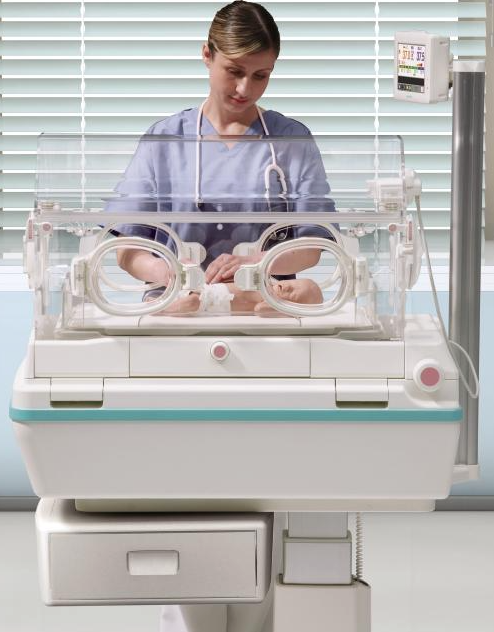
\includegraphics[width=.4\textwidth]{pics/isolette.png}
%\end{center}
%\caption{Isolette}
%\label{fig:isolette}
%\end{figure}

\newpage


\section{Context Diagram}
 
See Fig. A-1 in \cite{REMH}. The System Under Description (SUD) is a computer \emph{controller} to regulate the temperature of the Isolette. Everything else including the Operator Interface (described in \cite{REMH}) is in the ecosystem (i.e. in the environment of the controller). The monitored variables and controlled variables for the controller are in Table~\ref{table:monitored} and 
Table~\ref{tbl:cv}, respectively. For clarity, simplicity and safety, there are some differences between the specifications in this document and the descriptions in \cite{REMH}.\footnote{%
Documented in the write-up to this assignment: \texttt{assign1-spec.pdf}.} 

The differences in the SUD include, it will display an error message as well as the temperature back to the nurse at their station (see \emph{\cv{ms}} in table~\ref{tbl:cv}). The SUD will also employ an alarm as priority when the temperature becomes undesirable (set by the nurse, see \mv{al} in table~\ref{table:monitored}). Finally the SUD will keep track of the Isolette's state, that is it will have more states than the nurse can set (see \emph{\cv{md}} in table~\ref{tbl:cv}). For updated context diagram, see Fig.\ref{fig:modes}.

\newpage

\section{Goals}

The high-level goals (G) of the system are:

\begin{mylist}
\item G1---The Infant should be kept at a safe and comfortable temperature.

\item G2---The Nurse should be warned if the Infant becomes too hot or too cold.

\item G3---The cost of manufacturing the computer controller for the thermostat should be as low as possible.
\end{mylist}

\newpage
\hl{todo}
\section{Monitored Events}

The monitored events are those which come through the user interface. The following monitored events will be available to the user.

\begin{table}[h]
\centering
\begin{tabular}{|l|l|}
\hline
Name                                                                                                      & Interpretation                                                                           \\ \hline
\begin{tabular}[c]{@{}l@{}}add\_physician(id: ID\_MD; \\ name: NAME; kind: PHYSICIAN\_TYPE)\end{tabular}  & Add a Physician to the system                                                            \\ \hline
add\_patient(id: ID\_PT; name: NAME)                                                                      & Add Patient to the system                                                                \\ \hline
\begin{tabular}[c]{@{}l@{}}add\_medication(id: ID\_MN; \\ medicine: MEDICATION)\end{tabular}              & Add a medication to the system,                                                          \\ \hline
add\_interaction(id1:ID\_MN;id2:ID\_MN)                                                                   & \begin{tabular}[c]{@{}l@{}}Add an interaction between\\ two medications\end{tabular}     \\ \hline
\begin{tabular}[c]{@{}l@{}}new\_prescription(id: ID\_RX; \\ doctor: ID\_MD; patient: ID\_PT)\end{tabular} & \begin{tabular}[c]{@{}l@{}}Add a new prescription to \\ the system\end{tabular}          \\ \hline
\begin{tabular}[c]{@{}l@{}}add\_medicine(id: ID\_RX; \\ medicine:ID\_MN; dose: VALUE)\end{tabular}        & Add a medicine to a prescription                                                         \\ \hline
\begin{tabular}[c]{@{}l@{}}remove\_medicine(id: ID\_RX; \\ medicine:ID\_MN)\end{tabular}                  & \begin{tabular}[c]{@{}l@{}}Remove a medication from\\ a prescription\end{tabular}        \\ \hline
prescriptions\_q(medication\_id: ID\_MN)                                                                  & \begin{tabular}[c]{@{}l@{}}Get all the prescriptions with\\ that medication\end{tabular} \\ \hline
dpr\_q                                                                                                    & \begin{tabular}[c]{@{}l@{}}Get all the dangerous interactions\\ prescribed\end{tabular}  \\ \hline
\end{tabular}
\caption{Monitored Events}
\label{table:monitored}
\end{table}

\begin{table}[h]
\centering
\begin{tabular}{|l|l|l|}
\hline
Name            & Type                                                                                           & Interpretation                                                                                   \\ \hline
PHYSICIAN\_TYPE & \{gn, sp\}                                                                                     & \begin{tabular}[c]{@{}l@{}}Constrained to either \\ generalist or specialist\end{tabular}        \\ \hline
MEDICATION      & \begin{tabular}[c]{@{}l@{}}{[}name: NAME; kind: KIND; \\ low: VALUE; hi: VALUE{]}\end{tabular} & Constrained by GUI                                                                               \\ \hline
KIND            & \{pill, liquid\}                                                                               & \begin{tabular}[c]{@{}l@{}}Constrained to either \\ pill or a liquid\end{tabular}                \\ \hline
DOSE            & \{mg, cc\}                                                                                     & \begin{tabular}[c]{@{}l@{}}Constrained to either milligrams \\ or cubic centimetres\end{tabular} \\ \hline
\end{tabular}
\caption{Monitored Types}
\label{table:monitored-types}
\end{table}

\newpage

\hl{todo}
\section{Controlled Variables}
The controlled variables represent what will be shown to the user.

\begin{table}[h]
\centering
\begin{tabular}{|l|l|l|}
\hline
Name          & Interpretation                                             & Abstract State \\ \hline
Physicians    & A list of all the Physicians currently within the system   & See table \ref{abs-state}  \\ \hline
Patients      & A list of all the Patients currently in the system         & See table \ref{abs-state}  \\ \hline
Medications   & A list of all the Medications currently within the system  & See table \ref{abs-state}  \\ \hline
Interactions  & A list of all the Interactions currently within the system & See table \ref{abs-state}  \\ \hline
Prescriptions & A list of all the Prescriptions within the system          & See table \ref{abs-state}  \\ \hline
Error         & A message displaying the highest priority error, or ok     & See table \ref{abs-state}  \\ \hline
\end{tabular}
\caption {Controlled Variables}
\label{tbl:cv}
\end{table}

\newpage
\section{Mode Diagram}

REQ\ref{R1} states The \emph{controller} shall operate in one of four modes: \emph{off}, \emph{init}, \emph{normal} and \emph{fail}, shown in Fig.~\ref{fig:sc}. As shown in the figure, the Isolette will begin in the \emph{off} mode, and will enter \emph{init} mode when the nurse flips \mv{sw} into the \emph{on} position. The Isolette will only be able to move from the \emph{init} mode ot the \emph{normal} mode if it is properly configured such that the desired range is valid and not overlapping with the alarm levels, and both the sensors and operator controls are working (see REQ\ref{R6}).
Once inside the \emph{normal} mode, the controller will move to the \emph{fail} mode if either the controls or sensor fails, as specified in REQ\ref{R5}, and will only return to the \emph{normal} mode once they are both working correctly (REQ\ref{R7}). In any of these states, if the nurse switches \mv{sw} to \emph{off} the controller will switch to the off mode (REQ\ref{R8}).

\begin{figure}[!htb]
\begin{mdframed}
\begin{center}
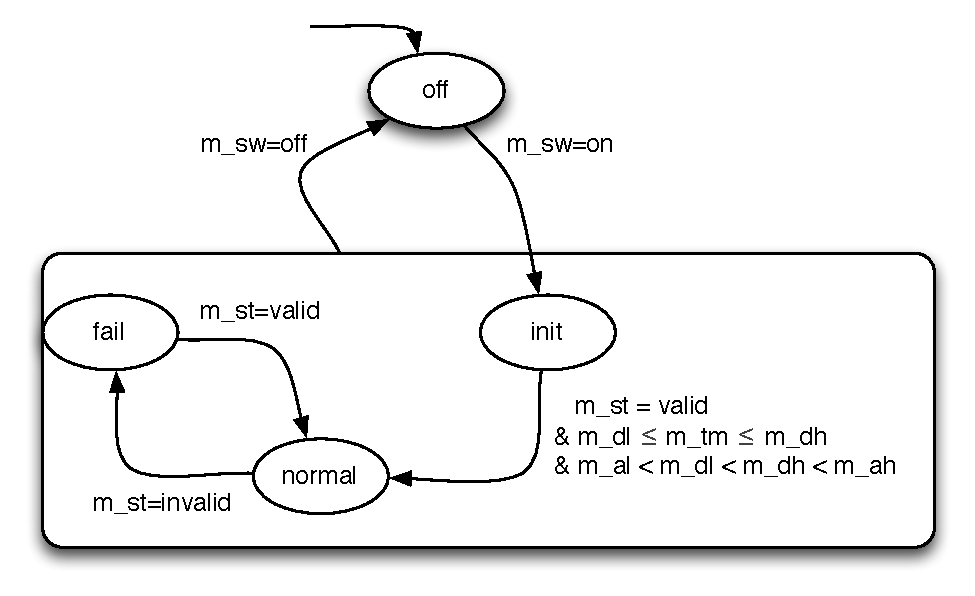
\includegraphics[width=.9\textwidth]{pics/mode-statechart.pdf}
\end{center}
\end{mdframed}
\caption{Statechart for the modes variable \cv{md}}
\label{fig:sc}
\end{figure}

\section{E/R-descriptions}

\subsection{Requirements Descriptions}
\reqm{REQ}
{The system will keep track of Physicians, Patients, Medications, and Prescriptions with unique IDs.\\~}
{ See Table~\ref{tbl:cv} for list of abstract states.\\}
\label{R1}
\textbf{Rationale:} Physicians and Patients may have non-unique names, and to avoid confusion when creating prescriptions, they must be identified by unique IDs. 

\reqm{REQ}
{The system will make a distinction between Physicians that are Generalists and Specialists.\\~}
{ See Table~\ref{table:monitored-types} for Monitored Types.\\}
\label{R2}
\textbf{Rationale:} The system will not allow \textit{Generalists} to add Medications to prescriptions where they may cause dangerous interactions. The assumption is made that \textit{Specialists} have received more training and it is left up to their discretion to allow Medications with dangerous Interactions to be prescribed.

\reqm{REQ}
{The system will only accept unique Medication names to prevent confusion.\\~}
{ Non-unique Medication names increase the chance of human error. \\}
\label{R3}
\textbf{Rationale:} Though Medications are also identified by a unique ID, it is critical that these are not mixed up, and as such it is required that the names are not identical as they may be for Patients or Physicians.

\reqm{REQ}
{The system will keep track of dangerous Interactions between Medications, as well as the order in which they were added.\\~}
{ Tracking dangerous Interactions allow for the system to properly flag them. \\}
\label{R4}
\textbf{Rationale:} The system must keep track of dangerous Interactions to enforce rules such as Generalists not being allowed to add Medications that case dangerous interactions. The client specified that they require the interactions within a prescription to be output in the order that the interactions were added to the system.

\reqm{REQ}
{The system will allow Physicians to prescribe Medications to Patients.\\~}
{ Basic functionality of a system tracking Prescriptions. \\}
\label{R5}
\textbf{Rationale:} The system is designed to keep track of Prescriptions between a Physician and a Patient.

\reqm{REQ}
{The system will allow Patients to have multiple Prescriptions, each with a unique Physician.\\~}
{ See Table~\ref{tbl:cv} for list of abstract states.\\}
\label{R6}
\textbf{Rationale:} The client has specified that Patients are not limited to one Physician, so they may have multiple Prescriptions. They will, however, have only one prescription per Physician.

\reqm{REQ}
{The system \textit{will not} allow a Generalist to add a Medication to a Prescription if the Medication leads to a dangerous Interaction. The system \textit{will} allow a Specialist to add a Medication to a Prescription if the Medication leads to a dangerous Interaction\\}
{ See Table~\ref{table:monitored} for adding medicine, and Table~\ref{tbl:cv} for dangerous interactions.\\~}
\label{R7}
\textbf{Rationale:} The system will prevent Generalists from adding Medications to Prescriptions where they may cause harm to the Patient. Specialists are  have more training, and therefore are determined to know what they are doing when prescribing such Medications.

\reqm{REQ}
{An interaction between two Medications cannot be added if both medications are prescribed to a patient
by generalists.\\}
{ See Table~\ref{table:monitored} for adding interaction, and Table~\ref{tbl:cv}.\\}
\label{R8}
\textbf{Rationale:} This critical safety requirement prevents a Generalist from being able to add dangerously interacting Medications to Prescriptions before the Interaction is added to the system. This requirement will prompt the user of the system to first remove one of the interacting Medications from the Prescription.

\reqm{REQ}
{A Medication may only be prescribed to a Patient once. \\}
{ A Medication may only be prescribed within the safe dosage range \\~}
\label{R9}
\textbf{Rationale:} This prevents different Physicians prescribing the same Medications and exceeding the safe dosage.

\subsection{Environmental Descriptions}
\reqm{ENV}
{All input to the system will be constrained to the input grammar.\\}
{ See Table~\ref{table:monitored} for the list possible monitored events.\\~}
\label{E1}

\reqm{ENV}
{Physicians and Patients may have identical names.\\}
{ We cannot control the names of people. They may have the same name. \\~}
\label{E2}

\reqm{ENV}
{Physicians are either \textit{Generalists} or \textit{Specialists}.\\}
{ See Table~\ref{table:monitored-types} for PHYSICIAN\_TYPE.\\~}
\label{E3}

\reqm{ENV}
{The DOSE type will be constrained by the GUI grammar to be either mg, or cc.\\}
{ See Table~\ref{table:monitored-types} for DOSE.\\~}
\label{E4}

\reqm{ENV}
{The KIND type will be constrained by the GUI grammar to be either a pill or a liquid.\\}
{ See Table~\ref{table:monitored-types} for KIND.\\~}
\label{E5}

\newpage
%%%%%%%%%%%%%%%%%%%%%%%%%%%%
\section{Abstract variables needed for the Function Table}

\begin{figure}[!htb]
\begin{center}
\begin{tabular}{|l|l|}
\hline
Name      & Conditional                                                       \\ \hline
$c1(i)$     & $\mv{st(i)} = valid$                                                  \\ \hline
$c2(i)$     & $\mv{dl(i)} \le \mv{tm(i)} \le \mv{dh(i)} $\\ \hline
$c3(i)$     & $\mv{al(i)}\,\textless\,\mv{dl(i)}\,\textless\,\mv{dh(i)}\,\textless\,\mv{ah(i)}$ \\ \hline
$c4(i)$     & $c1(i) \land c2(i) \land c3(i) $\\ \hline
$c5(i)$     & $\mv{tm(i)}\,\le\,\mv{al(i)} + 0.5$\\ \hline
$c6(i)$     & $\mv{tm(i)}\,\ge\,\mv{ah(i)} - 0.5$\\ \hline
$c7(i)$     & $c1(i) \land c3(i) \land \mv{al(i)}\,\textless\,\mv{tm(i)}\,\textless\,\mv{ah(i)}$\\ \hline
$c8(i)$     & $\neg c1(i) \lor \neg c3(i) \lor c5(i) \lor c6(i)$\\ \hline
$held\_for(i)$ & $(\forall\,(j: int): i - 10 \le j \land 0 \le j \implies \cv{al(j)} = on)$\\ \hline
\end{tabular}
\caption{Abstract Variables used in Function Tables}
\label{abs-state}
\end{center}
\end{figure}




\section{Function Tables}
%%%%%%%%%%%%%%%%%%%%%%%%%%%
\subsection{Function Table for Heat Control: \cv{hc}}
\begin{figure}[!htb]
\begin{center}
\begin{tabular}{|l|l|l|l|l|}
\hline
\multicolumn{4}{|l|}{Monitored Inputs \cv{md(i)}} & c\_hc(i) \\ \hline
\multicolumn{4}{|l|}{$i = 0$}& off \\ \hline
\multirow{4}{*}{$i\,\textgreater\,0$} & \multicolumn{3}{l|}{$c\_md(i) = off \lor \neg c1 \lor \neg c3$}& off      \\ \cline{2-5} 
& \multirow{3}{*}{$\neg c\_md(i) = off \land c1 \land c3$} & \multicolumn{2}{l|}{c2}                            & NC       \\ \cline{3-5} 
&                                                  & \multicolumn{2}{l|}{$m\_tm(i)\,\textless\,m\_dl(i)$}    & on       \\ \cline{3-5} 
& & \multicolumn{2}{l|}{$m\_tm(i)\,\textgreater\,m\_dh(i)$} & off      \\ \hline
\end{tabular}
\caption{Function Table for heat control: \cv{hc}}
\label{c_hc_ft}
\end{center}
\end{figure}

\newpage
%%%%%%%%%%%%%%%%%%%%%%%
\subsection{Function Table for Temperature Display: \cv{td}}
\begin{figure}[!htb]
\begin{center}
\begin{tabular}{|l|l|}
\hline
Monitored Inputs \mv{tm(i)}, \cv{md(i)} & \cv{td(i)} \\ \hline
$\cv{md(i)} = normal$         & \mv{tm(i)}    \\ \hline
$\neg \cv{md(i)} = normal$    & 0        \\ \hline
\end{tabular}

\caption{Function Table for Temperature Display: \cv{td}}
\label{c_td_ft}
\end{center}
\end{figure}

%%%%%%%%%%%%%%%%%%%%%%%
\subsection{Function Table for Mode: \cv{md}}
\begin{figure}[!htb]
\begin{center}
\begin{tabular}{|l|l|l|l|l|}
\hline
\multicolumn{4}{|l|}{Monitored Inputs \mv{sw(i)}, \cv{md(i-1)}} & \cv{md(i)}          \\ \hline
\multicolumn{4}{|l|}{$i=0$} & off    \\ \hline
\multirow{6}{*}{$i\,\textgreater\,0$} & \multicolumn{3}{l|}{\mv{sw(i)} = off}  & off    \\ \cline{2-5} 
                                & \multirow{5}{*}{\mv{sw(i)} = on} & \multicolumn{2}{l|}{$\cv{md(i-1)} = off$} & init  \\ \cline{3-5} 
                                &                              & \multirow{2}{*}{$\cv{md(i-1)} = normal \lor \cv{md(i-1)} = failed$} & $c1(i)$ & normal \\ \cline{4-5} 
                                &                              & & $\neg\,c1(i)$  & failed \\ \cline{3-5} 
                                &                              & \multirow{2}{*}{$\cv{md(i-1)} = init$}& $c4(i)$ & init \\ \cline{4-5} 
                                &                              &  & $\neg\,c4(i)$     & normal  \\\hline
\end{tabular}
\caption{Function Table for Mode: \cv{md}}
\label{c_md_ft}
\end{center}
\end{figure}

%%%%%%%%%%%%%%%%%%%%%%%
\subsection{Function Table for Messages: \cv{ms}}

\begin{figure}[!htb]
\begin{center}
\begin{tabular}{|l|l|}
\hline
Monitored Inputs \mv{al(i)}, \mv{ah(i)}, \mv{tm(i)} & \cv{ms(i)}         \\ \hline
$\neg\,c1(i)$ & invalid \\ \hline
$\neg\,c3(i)$ & config \\ \hline
$\mv{tm(i)} \,\textless\,\mv{al(i)}$ & low \\ \hline
$\mv{tm(i)}\,\textgreater\,\mv{ah(i)}$ & high \\ \hline
ELSE                                 & ok  \\ \hline
\end{tabular}
\caption{Function Table for Messages: \cv{ms}}
\label{c_ms_ft}
\end{center}
\end{figure}

\newpage
%%%%%%%%%%%%%%%%%%%%%%%
\subsection{Function Table for Alarm: \cv{al}}

\begin{figure}[!htb]
\begin{center}
\begin{tabular}{|l|l|l|l|l|}
\hline
\multicolumn{4}{|l|}{Monitored Inputs \mv{al(i)}, \mv{ah(i)}, \mv{tm(i)}} & \cv{al(i)}     \\ \hline
\multicolumn{4}{|l|}{$i = 0$} & off \\ \hline
\multirow{5}{*}{$i\,\textgreater\,0$} & \multirow{2}{*}{$\cv{al(i-1) = off}$} & \multicolumn{2}{l|}{$c7(i)$} & NC \\ \cline{3-5} 
                                &                                & \multicolumn{2}{l|}{$\neg c7(i)$} & on \\ \cline{2-5}
                                & \multirow{3}{*}{$\cv{al(i-1) = on}$} &   \multicolumn{2}{l|}{$c8(i)$} & NC \\ \cline{3-5} 
                                &                                & \multirow{2}{*}{$\neg c8(i)$} & $held\_for(i)$ & off  \\ \cline{4-5} 
                                &                                &                                    & $\neg held\_for(i) $ & on \\ \hline
                                
\end{tabular}
\caption{Function Table for Alarm: \cv{al}}
\label{c_al_ft}
\end{center}
\end{figure}

%%%%%%%%%%%%%%%%%%%%%%%%%%%%
\section{Validation}
\hl{todo}
\begin{figure}[!htb]
\begin{center}
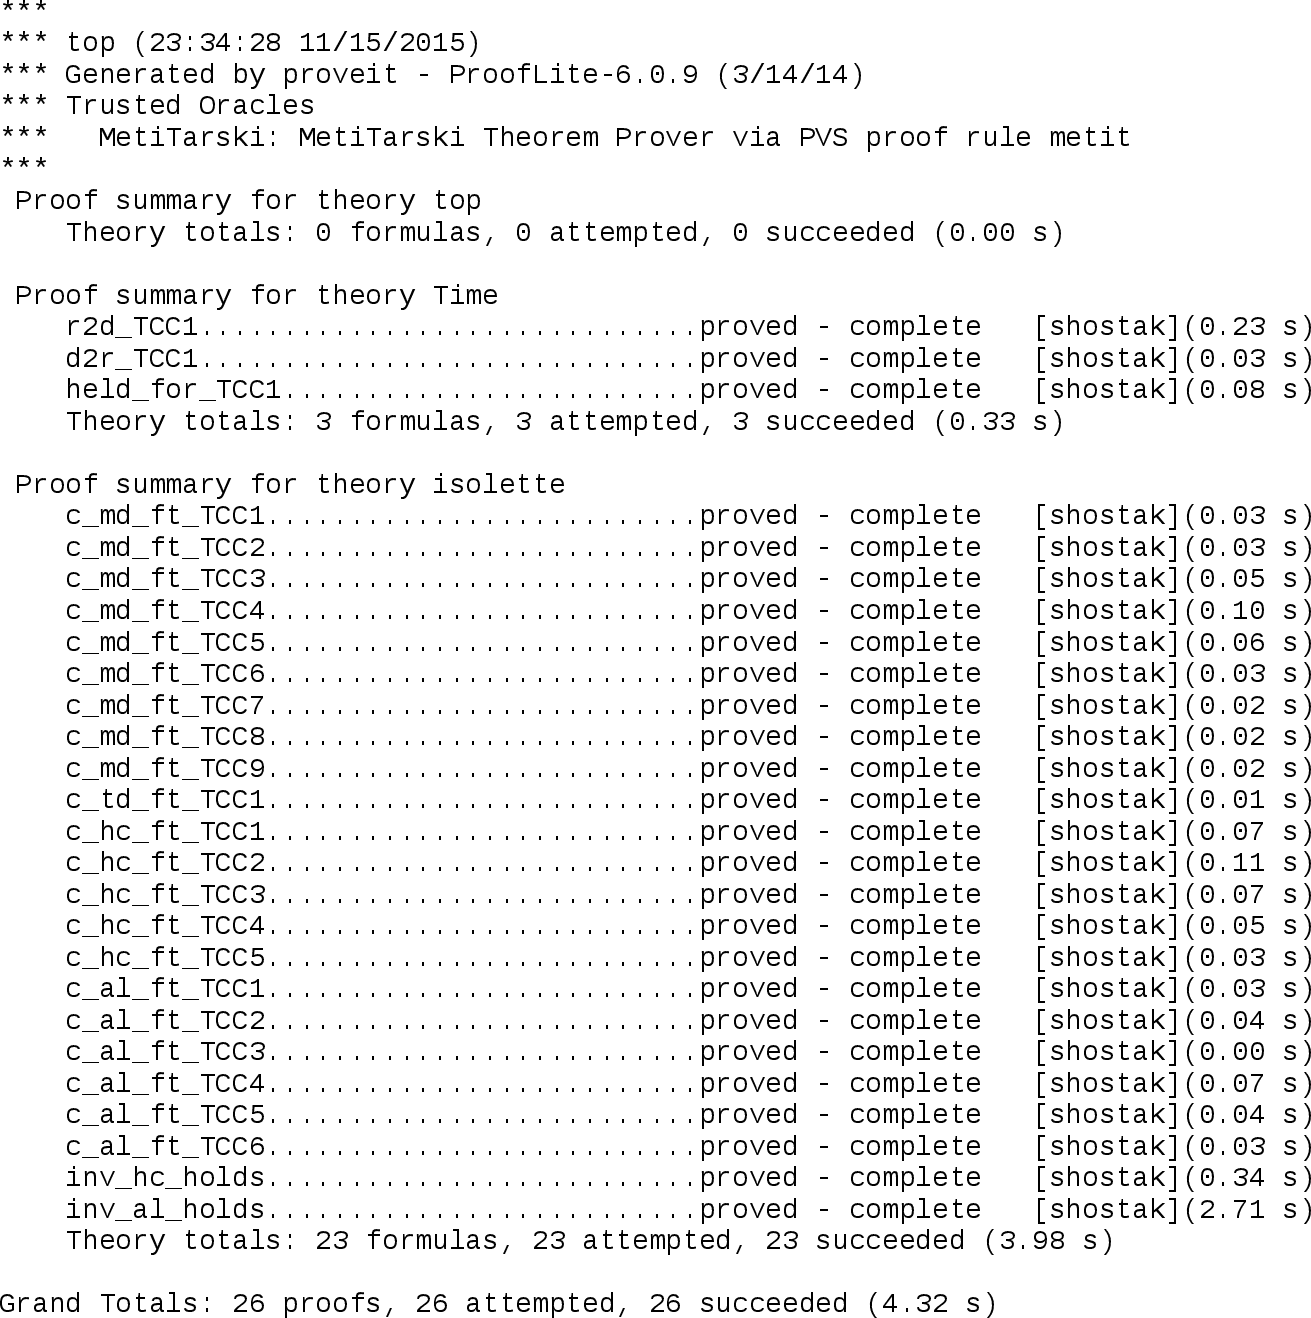
\includegraphics[width=1\textwidth]{pics/top.png}
\end{center}
\caption{Validated Isolette}
\label{proofs}
\end{figure}


You must also provide and prove in PVS one important safety invariant for the heat control $\cv{hc}$ and one important safety invariant for the alarm control \cv{al}.

Include the PVS sources in the appendix to this document but summarize the proofs here (top.summary).

\newpage 
\section{Use Cases}

See Section A2 of \cite{REMH} for some use cases. The use cases need to be adapted to the revised descriptions of the previous sections of this document.

\section{Acceptance Tests}

In this section, the use cases have to be converted into precise acceptance tests (using the function table to describe pre/post conditions) to be run when the design and implementation are complete.

\section{Traceability}

Matrix to show which acceptance tests passed, and which R-descriptions they checked.


\section{Glossary}

The definition of important terms is placed in this section. You are not required to complete this.
%%%%%%%%%%%%%%%%%%%%%%%%%%%%%%%%%%%%%
\newpage
\bibliographystyle{plain}
\bibliography{ref}

\newpage
\appendix 

\section{Additional Requirements}

\reqm{REQ}
{In \emph{fail} mode, the controller shall only return to \emph{normal} mode if
\begin{mylist}
\item The sensor is working and
\item The operator controls are working
\end{mylist}~}
{In \emph{fail} mode the controller shall return to \emph{normal} mode when \mv{st} returns ``valid"~\\}
\label{R7}

\reqm{REQ}
{In any mode, the controller will transition to the \emph{off} mode if the nurse turns the switch off.~\\}
{The controller will transition to \emph{off} mode from any mode if \mv{sw} becomes \emph{off}\\~}
\label{R8}


\newpage
\section{eHealth PVS}
\begin{pvs}
% This is a partial theory to help you get started encoding your
% function tables in PVS for the eHealth project.
% This theory type checks but the function tables are
% not valid as the requirements have not been properly elicited.
% Furthermore the function tables do not respect our format
% as completeness and disjointness is circumvented by the
% ELSE keyword.You may not use the ELSE keyword in function tables
% for this project.
% You are not required to prove any invariants.
% Nevertheless, we show you below how to prove some simple
% invariants as part of the state as TCCs. See fields inv1 and
% inv2 in the STATE record using the unit ADT. You may omit these
% invariants in the state if you choose, but they do help to ensure
% the correct requirements if kept.
% Note that we show a change of state using the override WITH
% operator so that any part of the state not overriden is left
% unchanged.

ehealth: THEORY
BEGIN
  delta: posreal % sampling time
  IMPORTING Time[delta]
  IMPORTING structures@Unit_adt
  i: VAR DTIME

  % Definition of an empty function
  emptyfun [T, U : TYPE] (x : {x : T | FALSE}) : RECURSIVE U =
    emptyfun(x)
    MEASURE (LAMBDA (x : {x : T | FALSE}): 1)

  ID_MD: TYPE+ = int %physicians
  ID_PT: TYPE+ = int %patients
  ID_RX: TYPE+ = int %prescriptions
  ID_MN: TYPE+ = int %medications

  % Physician type
  GS: TYPE+ = {gn, sp}
  UNIT: TYPE+ = {cc, mg}
  DOSE: TYPE = [nnreal, UNIT]
  NAME: TYPE+
  KIND: TYPE+ = {pill, liquid}

  MEDICINE: TYPE 
  = [name:NAME, kind:KIND, low:nnreal, hi:nnreal]

  COMMAND : DATATYPE
    BEGIN
      m_np(id:ID_RX, md: ID_MD, pt: ID_PT): np?
      m_ai(id1:ID_MN, id2:ID_MN): ai?
      m_am(id:ID_RX, med:ID_MN, dose:DOSE): am?
      m_rm(id:ID_RX, med: ID_MN): rm?
    END COMMAND
  cmd: VAR [POS_DTIME -> COMMAND]

  invariant (p : bool) : TYPE = { x : Unit | p }
  	    % unit : { x : Unit | 2 is even }
	    %  (type correct IFF: 2 is even [ x := unit ]
	    %  	     	     ...  2 is even
	    %		     	  TRUE
	    %
	    % unit : { x : Unit | 3 is even }
	    %  (type correct IFF: 3 is even [x := unit]
	    %  	     	     ...  3 is even
	    %		     	  FALSE
	    %
	    % { x : Unit | p } = IF p THEN {unit} ELSE {} ENDIF

  has [T : TYPE] (m : T, p : [T -> DOSE]) : bool = p(m)`1 > 0
      % does prescription p have a non-zero dose of m?

  % Have to place the state in a record
  STATE: TYPE =
    [#
        mnid: set[ID_MN]  % medication ids
      ,	ptid: set[ID_PT]  % patient ids
      , mdid: set[ID_MD]  % doctor ids
      ,	rxid: set[ID_RX]  % prescription ids
      , mdpt: set[[(mdid),(ptid)]] 
      % (doctor, patient) care relation
      , rx:   [(rxid) -> (mdpt)]   
      % care to rx ids,  needs to be a bijection
      , prs: [(rxid) -> [(mnid) -> DOSE]] 
      % prescriptions
      , di: set[[(mnid), (mnid)]]  
      , gs: [(mdid) -> GS] % kind of doctor
      , dpr : [(rxid) -> set[[(mnid), (mnid)]]]
   #]

  PRES (s : STATE) : TYPE =  [(s`mnid) -> DOSE]
       % type of PRESCRIPTIONS for a given state

  % would prescriptions p0 and p1 cause dangerous interactions
	% if they were prescribed to the same patient?
  interact (s : STATE)(p0, p1 : PRES (s)) : bool =
  	   EXISTS (m0,m1 : (s`mnid)):
	   	  s`di((m0,m1))
	      AND has(m0,p0)
	      AND has(m1,p1)

	  % given state s, does medication m1 cause a problem
	  % for the patient of prescription p0?
  interactWith (s: STATE)(p0 : PRES (s), m1 : (s`mnid)) : bool =
  	   EXISTS (m0 : (s`mnid)): s`di((m0,m1)) AND has(m0,p0)

	   medicine: MEDICINE
  isValidDose(s : STATE)(m : ID_MN, d : DOSE) : 
  bool = d`1 > 0 AND d`1 > medicine`3 AND medicine`4 > d`1
  	   % is d a valid dose of medication m?
	   % kept abstract; will need a counterpart in the state
	   % in order to be refined

  prsOfPt (s: STATE)(p: (s`ptid)) : set [(s`rxid)] =
  	  { r : (s`rxid) | s`rx(r)`2 = p }

  ptOf (s: STATE)(r : (s`rxid)) : (s`ptid) = s`rx(r)`2

  mdOf (s: STATE)(r : (s`rxid)) : (s`mdid) = s`rx(r)`1

  s: VAR [ DTIME -> STATE ]

  empty_prs (mdns : set[ID_MN])(m : (mdns)) : DOSE = (0, mg)

  init_mdid: set[ID_MD]
  init_gs: [(init_mdid) -> GS]
  init_mnid: set[ID_MN]
  init_ptid: set[ID_PT]
  init_rxid: set[ID_RX]
  init_mdpt: set[[(init_mdid),(init_ptid)]]
  init_dpr: [(init_rxid) -> set[[(init_mnid), (init_mnid)]]]
  init_prs: [(init_rxid) -> [(init_mnid) -> DOSE]] 
  init_rx: [(init_rxid)->(init_mdpt)]  

  init_state : STATE =
       (# mnid := init_mnid
        , ptid := init_ptid
        , mdid := init_mdid
        , rxid := init_rxid
       	, mdpt := init_mdpt 
        , rx := init_rx
        , prs := init_prs
        , di := emptyset
        , gs := init_gs
        , dpr := init_dpr
        #)

	% new_prescription (id: ID_RX; doctor: ID_MD;
	%		patient: ID_PT)
	%     prescription id must be a positive integer
	%     prescription id already in use
	%     physician id must be a positive integer
	%     physician with this id not registered
	%     patient id must be a positive integer
	%     patient with this id not registered
	%     prescription already exists for this physican
	%		and patient
  np_ft(id:ID_RX, md: ID_MD, pt: ID_PT)(s)(i): bool =
    COND
	i = 0 -> s(i) = init_state,
	i > 0 ->
	COND
	id > 0
	AND NOT rxid_ (id)
	AND md > 0
        AND mdid_ (md)
	AND pt > 0
        AND ptid_ (pt)
	AND mdpt_ (md, pt) ->
	       s(i) = s(i-1) 
	       WITH  [ rxid := add(id,rxid_)
		     , rx  := rx_ WITH [id := (md,pt)]
		     , prs := prs_ WITH [id := empty_prs(mnid_) ]
		     , dpr := dpr_ WITH [id := emptyset ] 
		    ] ,
        NOT (id > 0
        AND NOT rxid_ (id)
        AND md > 0
        AND mdid_ (md)
        AND pt > 0
        AND ptid_ (pt)
        AND mdpt_ (md, pt))
          -> s(i) = s(i-1)
    ENDCOND
    where
       rxid_ = s(i-1)`rxid
      ,mdid_ = s(i-1)`mdid
      ,ptid_ = s(i-1)`ptid
      ,mdpt_ = s(i-1)`mdpt
      ,rx_   = s(i-1)`rx
      ,dpr_  = s(i-1)`dpr
      ,mnid_ = s(i-1)`mnid
      ,prs_ = s(i-1)`prs
      ENDCOND      

%dose: DOSE
 % Add_medicine (id: ID_RX; medicine:ID_MN; dose: VALUE)
 %     prescription id must be a positive integer
 %     prescription with this id does not exist
 %     medication id must be a positive integer
 %     medication id must be registered
 %     medication is already prescribed
 %     specialist is required to add a dangerous interaction
 %     dose is outside allowed range
  am_ft(id:ID_RX, m: ID_MN, d: DOSE)(s)(i): bool =
    COND
	i = 0 -> s(i) = init_state,
        i > 0 -> COND
	id > 0 
	AND rxid_ (id)
	AND m > 0 
	AND mnid_ (m)
	AND NOT (prs_ (id)(m)`1 > 0)
	AND NOT (EXISTS (b: ID_MD, c: ID_PT): 
	((prs_ (id)(m)`1 > 0 AND (rx_ (id) = (b,c) 
	AND gs_ (b) = sp ))))
	AND isValidDose_ (m,d)
            -> s(i) = s(i-1) WITH [ prs := prs_ 
            WITH [id := prs_(id) WITH [m := d] ] ]
     , NOT(	id > 0 
	AND rxid_ (id)
	AND m > 0 
	AND mnid_ (m)
	AND NOT (prs_ (id)(m)`1 > 0)
	AND NOT (EXISTS (b: ID_MD, c: ID_PT): 
	((prs_ (id)(m)`1 > 0 AND (rx_ (id) = (b,c) 
	AND gs_ (b) = sp ))))
	AND isValidDose_ (m,d))
        -> s(i) = s(i-1)
    ENDCOND
    where
       rxid_ = s(i-1)`rxid
      ,mnid_ = s(i-1)`mnid
      ,di_ = s(i-1)`di
      ,rx_ = s(i-1)`rx
      ,gs_ = s(i-1)`gs
      ,prs_  = s(i-1)`prs
      ,mdOf_ = mdOf(s(i-1))
      ,ptOf_ = ptOf(s(i-1))
      ,interactWith_ = interactWith(s(i-1))
      ,prsOfPt_ = prsOfPt(s(i-1))
      ,isValidDose_ = isValidDose(s(i-1))
      ENDCOND

%%%%%%%%%%%%%%%%%%%%%%%%%%%%%
%% FUN FUN FUNCTION TABLES %%
%%%%%%%%%%%%%%%%%%%%%%%%%%%%%

      %add_interaction (id1:ID_MN;id2:ID_MN)
      %    medication ids must be positive integers
      %    medication ids must be different
      %    medications with these ids must be registered
      %    interaction already exists
      %    first remove conflicting medicine prescribed by
      %	generalist
      ai_ft(id1:ID_MN, id2:ID_MN)(s)(i): bool = COND
          i = 0 -> s(i) = init_state,
          i > 0 -> COND
	  id1 > 0 AND id2 > 0
          AND NOT (id1 = id2)
	  AND member(id1, mnid_ )
	  AND member(id2, mnid_ )
	  AND NOT member((id1,id2), di_ )
          AND NOT (EXISTS (a: ID_RX, b: ID_MD, c: ID_PT): 
          member(a, rxid_ ) AND member(b, mdid_ ) 
          AND member(c, ptid_ ) AND ((prs_ (a)(id1)`1 > 0 
          AND (rx_ (a) = (b,c) AND gs_ (b) = sp )) 
	      OR (prs_ (a)(id2)`1 > 0 AND (rx_ (a) = (b,c) 
	      AND gs_ (b) = sp))))
   	 AND NOT (member((id1, id2), di_ )                                             
            OR member((id2, id1), di_ ))
	  -> s(i) = s(i-1) WITH [
              di := add((id1, id2), di_ )
              ,di := add((id2, id1), di_ )
	     % ,dpr := dpr_ WITH []
          ],
          NOT (
            id1 > 0 AND id2 > 0
          AND NOT (id1 = id2)
          AND member(id1, mnid_ )
          AND member(id2, mnid_ )
          AND NOT member((id1,id2), di_ )
          AND NOT (EXISTS (a: ID_RX, b: ID_MD, c: ID_PT):
           member(a, rxid_ ) AND member(b, mdid_ ) 
           AND member(c, ptid_ ) AND ((prs_ (a)(id1)`1 > 0 
           AND (rx_ (a) = (b,c) AND gs_ (b) = sp ))
              OR (prs_ (a)(id2)`1 > 0 AND (rx_ (a) = (b,c) 
              AND gs_ (b) = sp))))
         AND NOT (member((id1, id2), di_ )
            OR member((id2, id1), di_ )) ) -> s(i) = s(i-1)
      ENDCOND
      where
        di_   = s(i-1)`di
        ,dpr_  = s(i-1)`dpr
	,rxid_ = s(i-1)`rxid
        ,mnid_ = s(i-1)`mnid
	,mdid_ = s(i-1)`mdid
	,ptid_ = s(i-1)`ptid
        ,prs_  = s(i-1)`prs
	,rx_ = s(i-1)`rx
	,mdpt_ = s(i-1)`mdpt
	,gs_ = s(i-1)`gs
	ENDCOND
      %remove_medicine  (id: ID_RX; medicine:ID_MN)
      %    prescription id must be a positive integer
      %    prescription with this id does not exist
      %    medication id must be a positive integer
      %    medication id must be registered
      %    medication is not in the prescription
      rm_ft(id:ID_RX, med: ID_MN)(s)(i): bool = COND
          i = 0 -> s(i) = init_state,
        i > 0 -> COND
	   id > 0
	  AND rxid_ (id)
	  AND med > 0
	  AND mnid_ (med)
	  AND prs_ (id)(med)`1 > 0
	  -> s(i) = s(i-1) WITH [
	    prs := prs_ WITH [id := empty_prs(mnid_ ) ]
	  ],
          NOT (
            id > 0
	    AND rxid_ (id)
            AND med > 0
            AND mnid_ (med)
            AND prs_ (id)(med)`1 > 0
          ) -> s(i) = s(i-1)
      ENDCOND
      where
         rxid_ = s(i-1)`rxid
        ,dpr_  = s(i-1)`dpr
        ,mnid_ = s(i-1)`mnid
        ,prs_  = s(i-1)`prs
	ENDCOND

ehealth_ft(cmd)(s)(i): bool = COND
  i = 0 -> s(0) = init_state,
  i > 0 ->
    CASES cmd(i) OF
      m_np(id, md, pt):  np_ft(id, md, pt)(s)(i),
      m_ai(id1, id2): ai_ft(id1, id2)(s)(i),
      m_am(id, med, dose): am_ft(id, med, dose)(s)(i),
      m_rm(id, med): rm_ft(id, med)(s)(i)
    ENDCASES
ENDCOND

END ehealth
\end{pvs}

\end{document}  
